\documentclass{article}

\usepackage{graphicx}
\usepackage[margin=1in]{geometry}
\usepackage{float}
\usepackage[hidelinks]{hyperref}

\begin{document}

\title{Radial Single-Kernel fi Optimization Report}
\author{}
\date{19 March 2026}
\maketitle
\footnotesize
\setlength{\parindent}{0pt}

This report summarizes the radial single-kernel notebook and the later constrained version that was added to make the kernel shape more meaningful.

\section*{Results from the Notebook}
Original radial fit (\texttt{abs\_max}, outer radii frozen to seed):

Val: AUC \texttt{0.8898}, accuracy at \texttt{0.5} = \texttt{0.8182}.

Test: AUC \texttt{0.8825}, accuracy at \texttt{0.5} = \texttt{0.8000}

Learned radial kernel:

Val: AUC \texttt{0.9189}, accuracy at \texttt{0.5} = \texttt{0.8545}

Test: AUC \texttt{0.9286}, accuracy at \texttt{0.5} = \texttt{0.8668}

\begin{figure}[H]
    \centering
    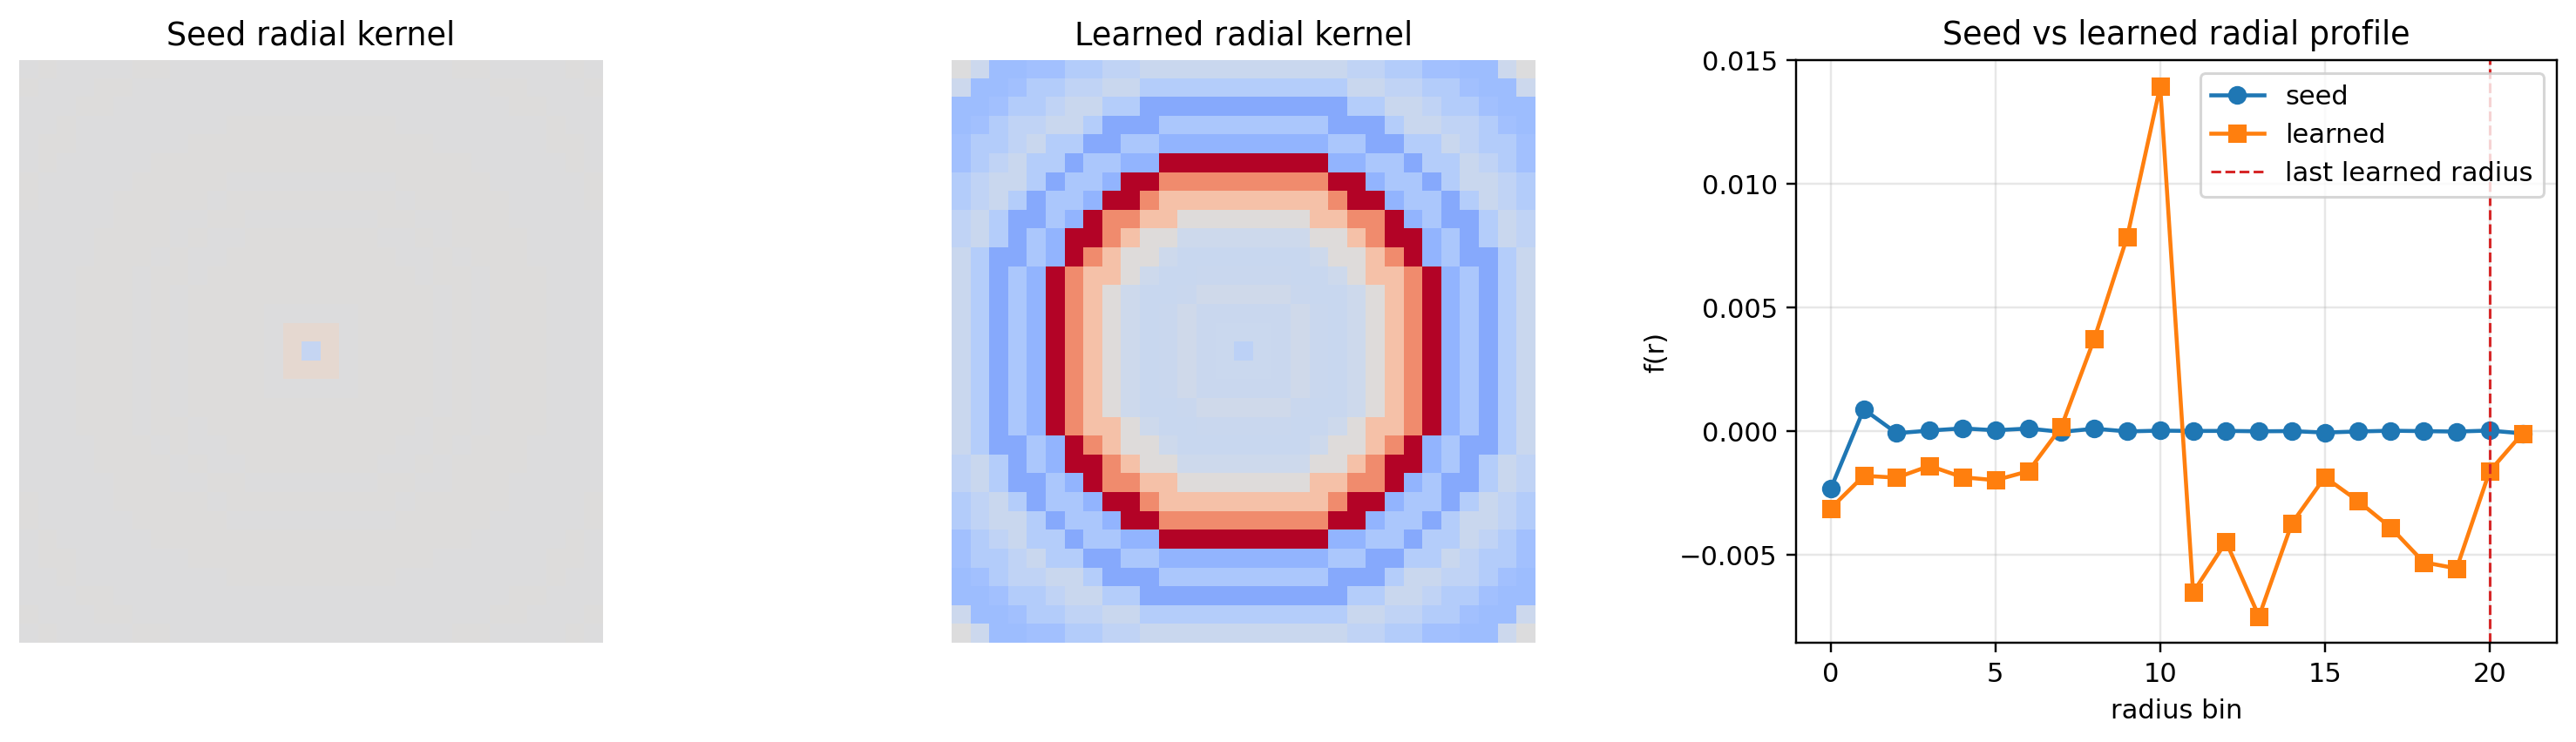
\includegraphics[
        width=0.98\textwidth,
        trim=0 0 0 0,
        clip
    ]{figures/radial_single_kernel_current_summary.png}
    \caption{Original learned radial kernel from the notebook with \texttt{fi} limit = 20.}
\end{figure}

\begin{figure}[H]
    \centering
    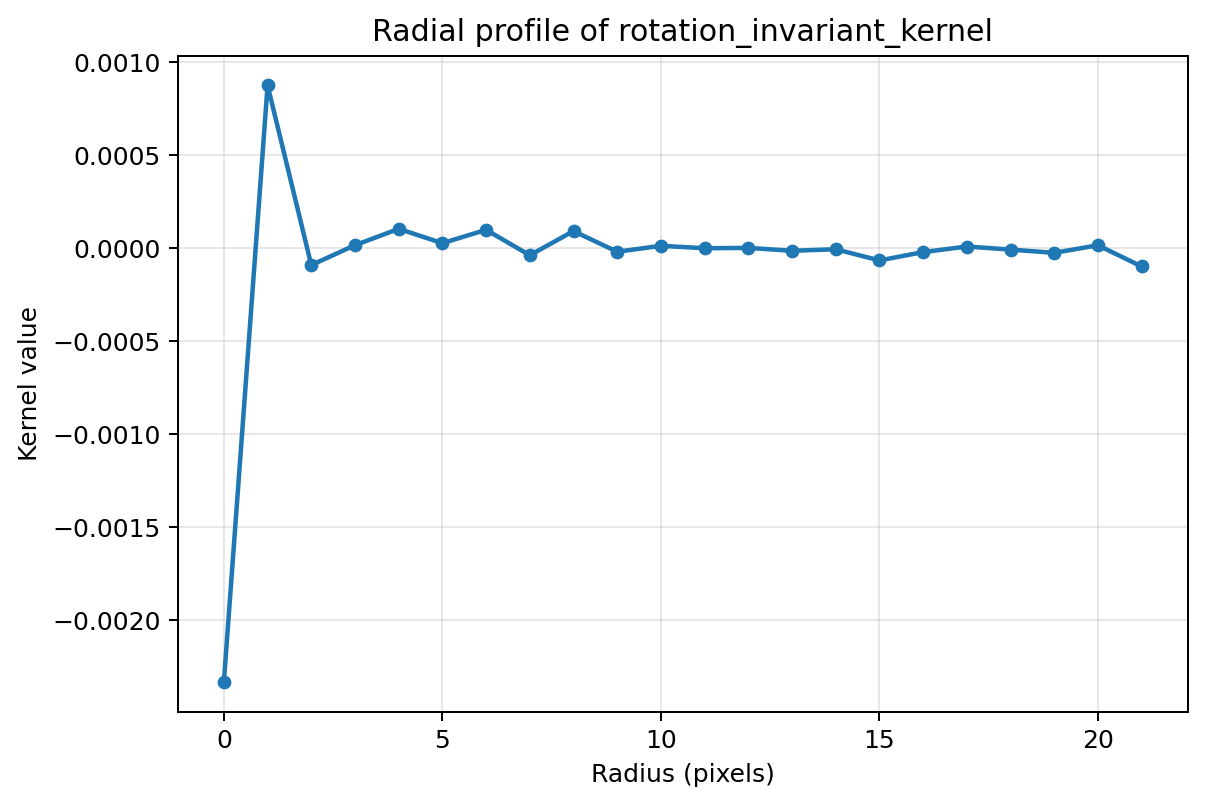
\includegraphics[width=0.42\textwidth]{figures/radial_single_kernel_rotation_invariant_profile.png}
    \caption{Radial profile of the original rotation-invariant kernel from 21st Feb report}
\end{figure}
The learned kernel has a similar starting shape (focused on 0 - 5) where it is increasing then decreasing and then plateaued.

\section*{Clarifications}
\textbf{Why does it look different from the earlier preset-family kernel?} \\
The earlier method was restricted by preset kernel families. This approach searches in a different space and learns completely free radial profile directly from data, so a different shape is expected.


\textbf{Why is the learned profile not always decreasing with radius?} \\
The original loss does not force the profile to decrease with radius. It only rewards what improves classification, and outer rings cover more pixels, so they can still receive large weight.


\textbf{Why can different runs give different kernels?} \\
The kernel is not uniquely determined by the classification loss. Several different radial profiles can give similar responses and similar accuracy, and this ambiguity becomes stronger when \texttt{abs\_max} removes sign information. (Added constraints to get a converging kernel in the next section)


% \textbf{My understanding about the non-decreasing kernel profile and does it mean the kernel is not finite?} \\
% The kernel is can be still considered finite because it lives on a fixed image window even if the profile is not strictly decreasing.

\section*{Changes to make the kernel converging}
The constrained version added four changes:
\begin{itemize}
    \item Replace \texttt{abs\_max} with a signed response.
    \item Zero out \texttt{r > Rmax} instead of freezing those radii to the seed.
    \item Add monotone and decay regularization.
    \item Normalize kernel scale and fix the sign convention.
\end{itemize}


\section*{Signed Compact Kernel Results}
Signed compact fit (\texttt{signed\_peak}, hard cutoff at \texttt{Rmax = 20}):

Val: AUC \texttt{0.8878}, accuracy at \texttt{0.5} = \texttt{0.8150}

Test: AUC \texttt{0.8808}, accuracy at \texttt{0.5} = \texttt{0.8011}

\begin{figure}[H]
    \centering
    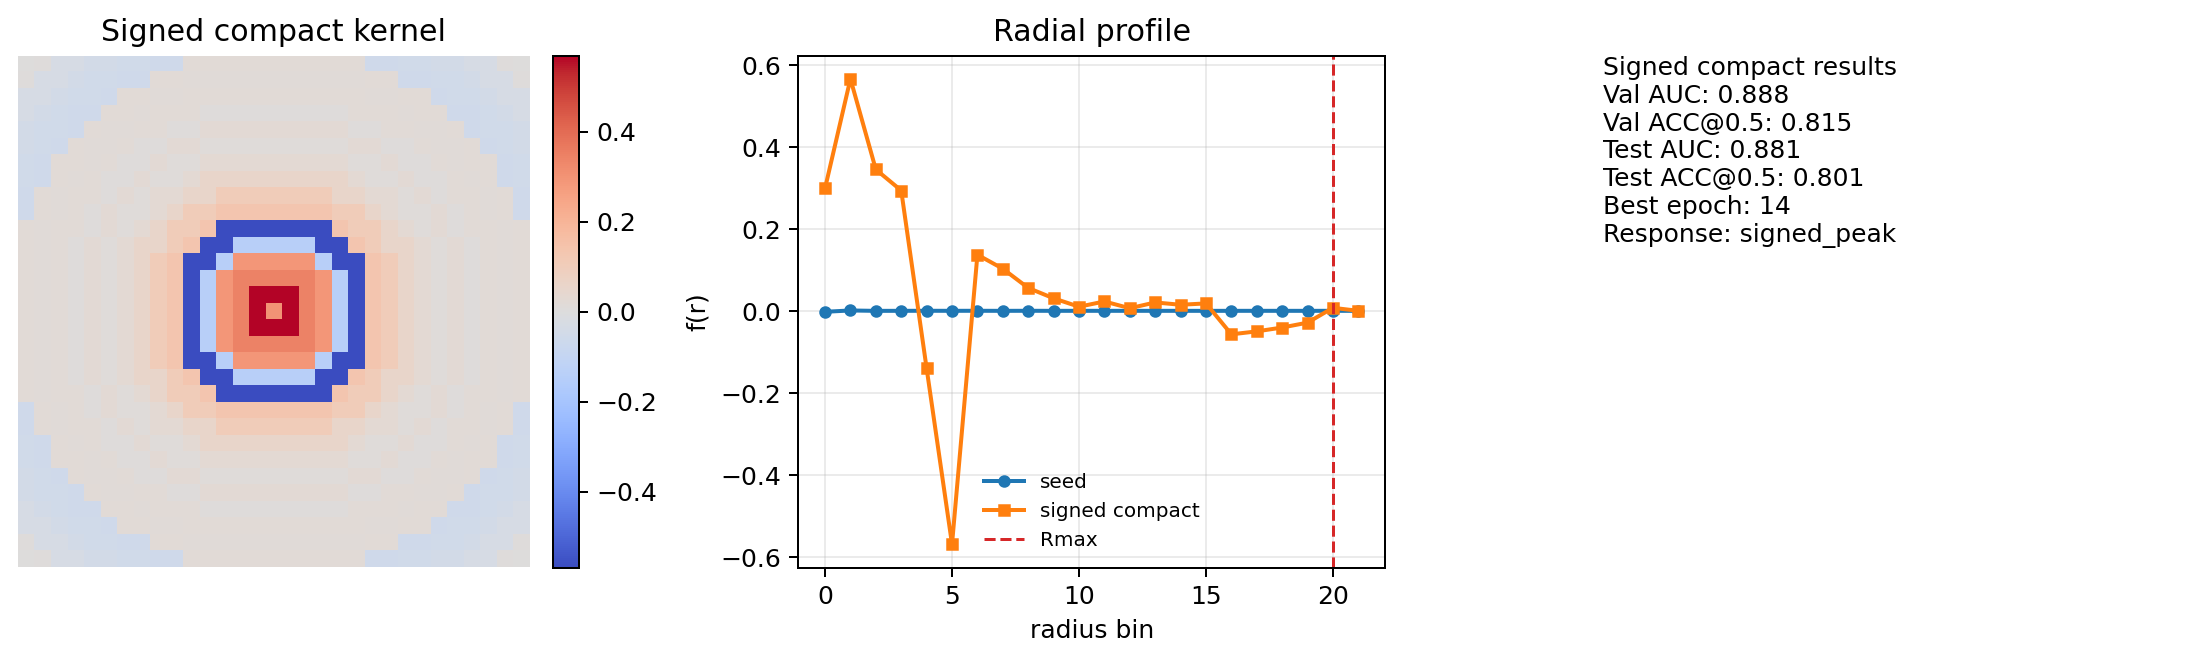
\includegraphics[width=0.88\textwidth]{figures/radial_single_kernel_signed_compact_summary.png}
    \caption{Final signed compact kernel and its radial profile. This is the constrained kernel used for the later exact heatmap.}
\end{figure}


\begin{figure}[H]
    \centering
    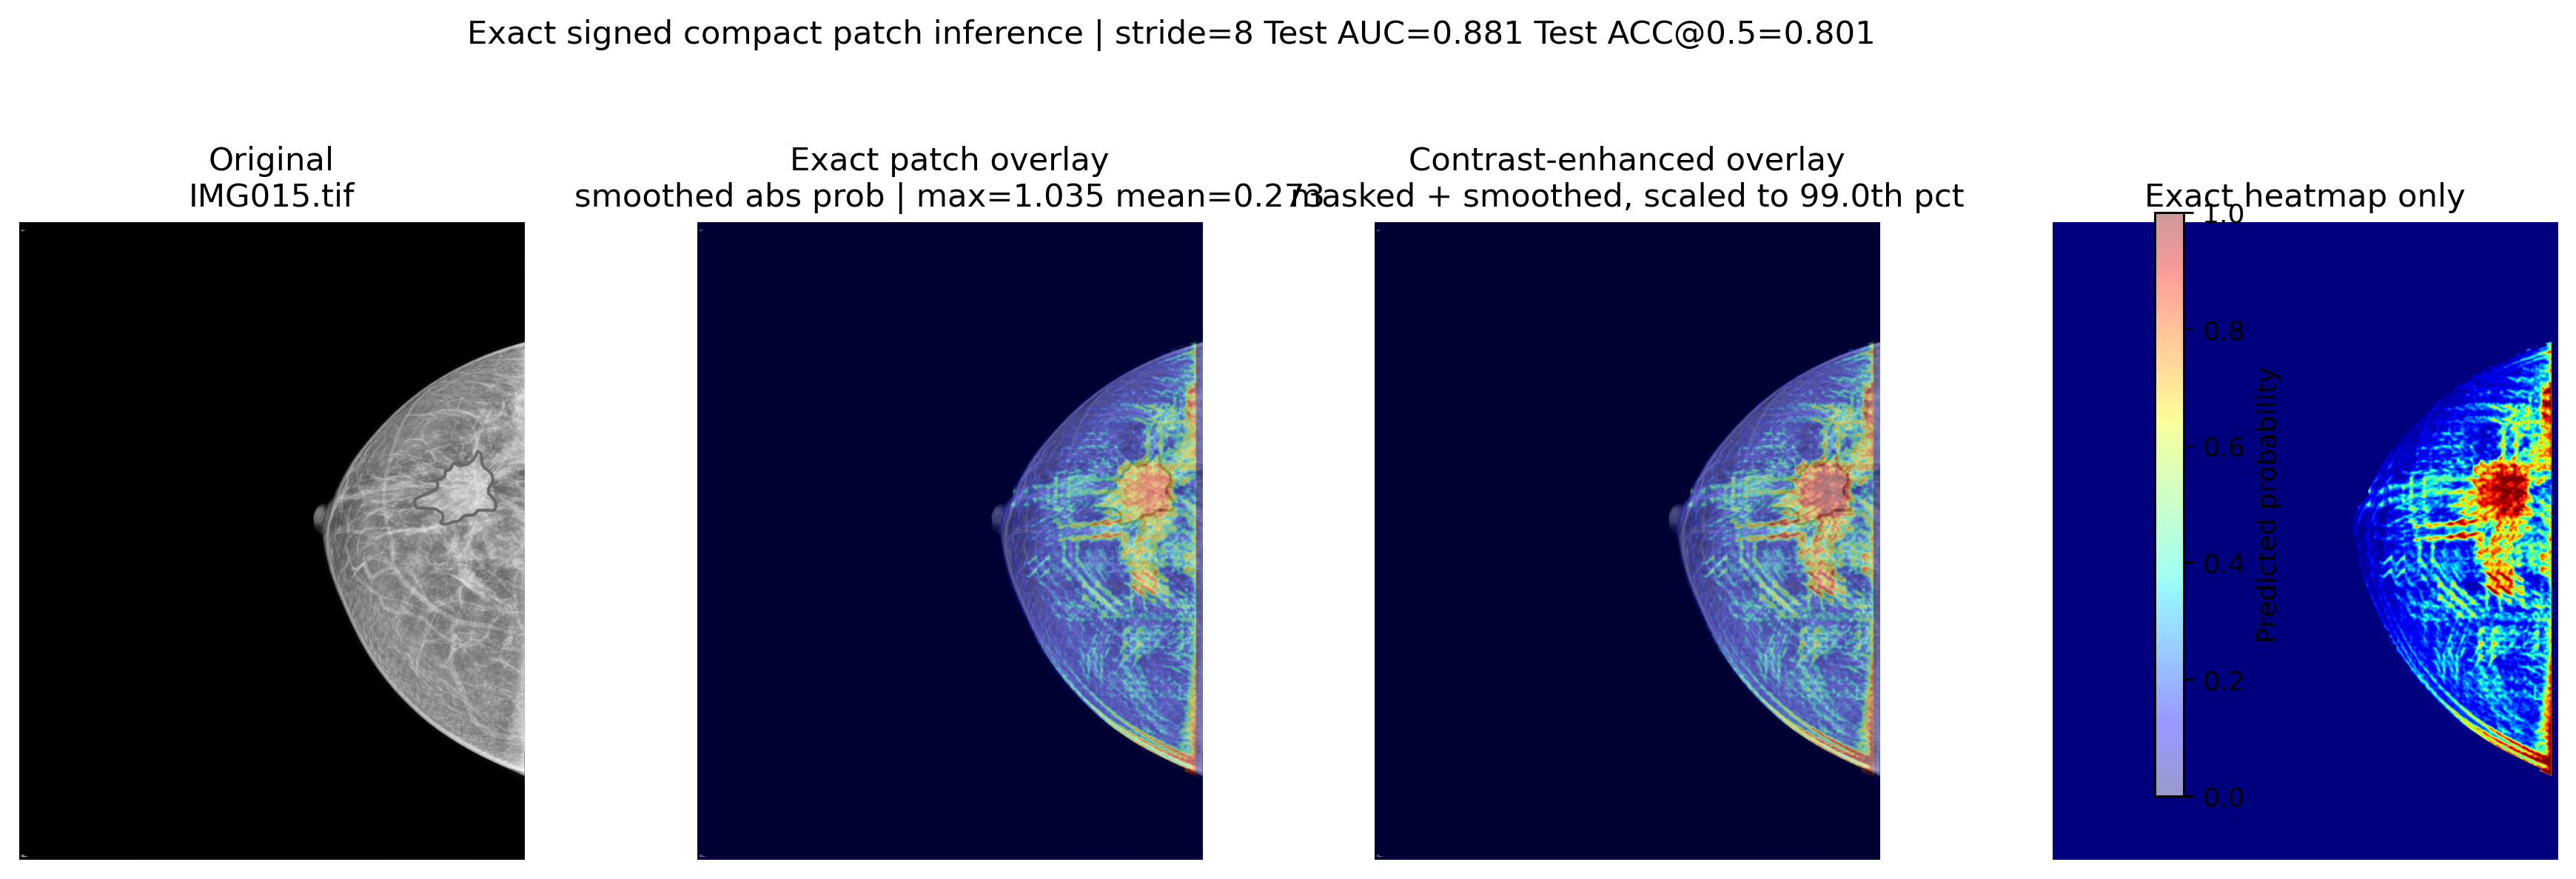
\includegraphics[width=0.88\textwidth]{figures/radial_single_kernel_signed_exact_heatmap.png}
    \caption{Heatmap of the signed compact kernel}
\end{figure}

\section*{Summary}
The original \texttt{abs\_max} radial fit gives the best classification numbers in this notebook, with test AUC \texttt{0.9286} and test accuracy \texttt{0.8668}. However, that setup does not identify a unique kernel shape very well. The later signed compact version gives slightly lower classification performance, with test AUC \texttt{0.8808} and test accuracy \texttt{0.8011}, but it makes the kernel itself easier to interpret because the response is signed, the support is explicitly limited, and the profile is regularized. 
\end{document}
